
\section{The Infomax Principle (Bell \& Sejnowski, 1995)}

\begin{itemize}
\item[\emph{Idea:}] Under certain conditions, maximizing the
  \emph{mutual information} between inputs (mixed signals $\vec x$) and outputs
  (recovered sources $\widehat{\vec s}$) of a system yields \emph{independent} outputs. 
  If sources are independent, then
  transformations of these sources are independent, too.
  
  Choosing the transformation such that their marginal distributions become uniform 
  simplifies the computations to find independent sources. i.e. choosing the transformation \\
$\widehat{u}_i = \widehat{f}_i(\widehat{s}_i)$ such that
$\widehat{P}_{u_i}(\widehat{u}_i) = \mathrm{const.}$

\end{itemize}

\underline{Recap on Density Transformations:}

The transformation is found using \emph{conservation of probability}
\begin{equation}
	\widehat{P}_{u_i}(\widehat{u}_i) d \widehat{u}_i 
	\; =  \; \widehat{P}_{s_i} (\widehat{s}_i) d \widehat{s}_i.
\end{equation}
Using the general rule for density transformations and applying it here yields
\begin{equation}
\label{eq:conservation1}
	\widehat{P}_{u_i}(\widehat{u}_i) \quad
	 =  \quad \bigg| 
		\frac{d \widehat{s}_i}{d \widehat{u}_i} \bigg| 
			 \widehat{P}_{s_i}(\widehat{s}_i) \quad
	 =  \quad \frac{1}{\big| \widehat{f}_i^{'} (\widehat{s}_i) \big|} 
		\widehat{P}_{s_i}(\widehat{s}_i)
\end{equation}
where $\left|\frac{d \widehat{s}_i}{d \widehat{u}_i} \right|$ is
called \emph{functional determinant} of the transformation
$\widehat{f}_i$.
Applying the principle of conservation of probability (equal size
areas) to find a transformation resulting in a uniformly distributed
variable with a constant density yields: 
\begin{equation}
  \label{eq:dtufs}
		\widehat{P}_{u_i} (\widehat{u}_i) \; = \;   
		 \frac{1}{\big| \widehat{f}_i^{'} (\widehat{s}_i) \big|} 
		\widehat{P}_{s_i}(\widehat{s}_i) \; \stackrel{!}{=} \; const \qquad \Rightarrow \qquad 
		 \big| \widehat{f}_i^{'} (\widehat{s}_i) \big| =  a \widehat{P}_{s_i}(\widehat{s}_i) 
\end{equation}
and therefore
\begin{equation}
\Rightarrow \widehat{f}_i (\widehat{s}_i)
 = \int\limits_{-\infty}^{\widehat{s}_i} dy\; a 
			\widehat{P}_{s_i}(y)
\end{equation}

\begin{figure}[h]
  \centering
  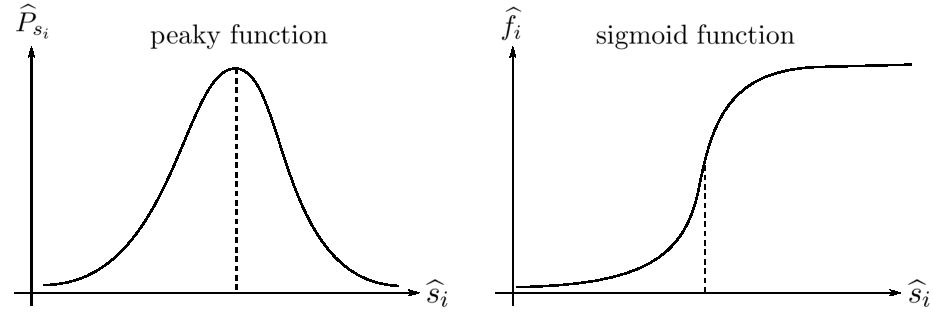
\includegraphics[width=12cm]{img/section2_fig15}  
  %\caption{density (pdf) and corresponding distribution function (cdf)}
  \label{fig:cdf}
\end{figure}

\newpage

\section{Approach 0: Maximizing mutual information directly}

Another way to reach the cost function is to maximize the mutual information directly:

$$
I(Y,X) = h(Y) - h(Y|X)
$$

By considering the following relationship between $Y$ and $X$:\\
$Y = g(X;w) + \mathcal{N}$, where $g(\cdot)$ is some invertible transformation parametrized by $w$ and $\mathcal{N}$ is additive noise.

By taking the derivative with respect to the parameter $w$:

$$
\frac{\partial}{\partial w} I(Y,X) = \frac{\partial}{\partial w}h(y) - 
\underbrace{\frac{\partial}{\partial w} h(Y|X)}_{= \frac{\partial}{\partial w} h(\mathcal{N}) = 0}
$$

Maximizing the $I(Y,X)$ boils down to maximizing the entropy of the output $Y$. 
We've seen how mutual information relates to the KL divergence, so we're going to use an approach 
that operates on the KL-divergence. 
Whether Infomax by maximizing entropy\footnote{if interested see Bell, A. J., \& Sejnowski, T. J. (1995). An information-maximization approach to blind separation and blind deconvolution. Neural computation, 7(6), 1129-1159.} 
or finding a factorization via the KL-divergence,
both are based on the Infomax principle and arrive at the same solution.

\clearpage

\section{Approach 1: Infomax via KL-divergence for the transformed densities}
\begin{eqnarray}
  \dkl & = & \int d \, \widehat{\vec{s}} P_{\vec{s}}(\widehat{\vec{s}}) \ln \frac{P_{\vec{s}}(\widehat{\vec{s}})}{\prod_i \widehat{P}_{s_i}(\widehat{s}_i)}\\
  & = &  \int d \, \widehat{\vec{s}} P_{\vec{s}}(\widehat{\vec{s}}) \ln 
  \frac
  {P_{\vec{s}}(\widehat{\vec{s}}) \quad \prod_i \frac{1}{f_i' (\widehat{s}_i)}}
  {\prod_i \widehat{P}_{s_i}(\widehat{s}_i) \quad \frac{1}{f_i' (\widehat{s}_i)}} \\
  & = & \int d \widehat{\vec{u}} P_{\vec{u}} (\widehat{\vec{u}}) 
  \ln 
  \frac
  {P_{\vec{u}} (\widehat{\vec{u}}) }
  {\prod_i  \widehat{P}_{u_i}(\widehat{u_i})} \\
  & = & 
  \underbrace{
	  \int d \widehat{\vec{u}} P_{\vec{u}} (\widehat{\vec{u}}) 
	  \ln 
	  {P_{\vec{u}} (\widehat{\vec{u}}) }
  }_{= -H \; \text{(negative entropy)}}\\
  & & \quad -
  \underbrace{
	  \int d \widehat{\vec{u}} P_{\vec{u}} (\widehat{\vec{u}}) 
	  \left( \ln
	  {\prod_{i=1}^{N}
	  \underbrace{ 
		\widehat{P}_{u_i}(\widehat{u_i}) 
	  }_{\substack{\text{const.\;} a \\\text{\;see \eqref{eq:dtufs}}}}} 
	  \right)
	  }_{\text{const.}}
\end{eqnarray}

This motivates the socalled \emph{Infomax principle}:
\begin{equation}\label{eq:infomax}
  H = -\int d \widehat{\vec{u}} P_{\vec{u}} (\widehat{\vec{u}})
  \ln P_{\vec{u}} (\widehat{\vec{u}}) \eqexcl \max 
\end{equation}
using the transformed estimated sources
\begin{equation}
\widehat{u}_i := \widehat{f}_i \big( \underbrace{ \vec{e}_i^\top
		\vec{W} \, \vec{x}  }_{= \widehat{s_i} } \big) 
\end{equation}

This tells us that we can produce statistally independent sources $\widehat {\vec s}$ 
by maixmizing the negative entropy of the of their transformation.\\
Now that we've found the cost function for our learning algorithm. 
How do we build something that can learn to solve it.

% -----------------------------------------------------------------------------
